Three 2D views are shown in the main window, corresponding to the axial, coronal
and sagittal views of the volume. On each view some information is
shown, such as the resolution of the slice (in pixels), the size of a voxel (in mm), the
index of the slice being shown, and the value of the pixel at the current selection). 
By default, a trilinear interpolation is made between pixels. Press
{\large \bf ``i''} to disable this interpolation.

\begin{figure}[htbp]
    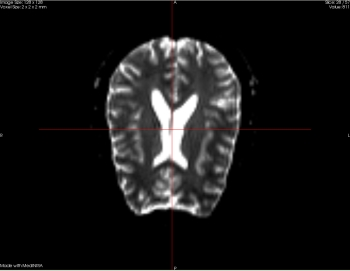
\includegraphics[width=0.32\linewidth]{2dview1}
    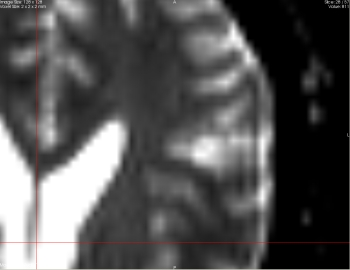
\includegraphics[width=0.32\linewidth]{2dview2}
    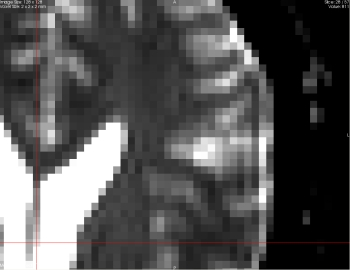
\includegraphics[width=0.32\linewidth]{2dview3}
  \caption{2D view navigation. On the left you see a 2D view (axial) centered on the
    screen. When the zoom interaction is selected, you can zoom in the view by moving
    the mouse up while left-clicking on the view and translate the view by
    middle-clicking (middle figure). You can disable the interpolation between pixel by
    pressing {\large \bf``i''} (right figure). Reset the image position by pressing
    {\large \bf``r''}.
  \label{fig:2dviewzoom}}
\end{figure}

\noindent 
\includegraphics[width=0.7cm]{selector}
Several mouse interactions are available. With the selection interaction (black arrow),
you will navigate in the volume (i.e. select a slice) by moving the mouse up or down
while left-clicking on a view. Press {\large \bf``r''} to reset the position to default.

\noindent 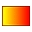
\includegraphics[width=1cm]{greyscale}
The second interaction (windowing) controls the brightness/contrast of the image by moving the
mouse while left-clicking on the view. A left-right movement controls contrast while up-down
controls brightness. Note that with these two interactions, the 4 different views are
synchronized. Press {\large \bf``r''} to reset the contrast to default value.

\noindent 
\includegraphics[width=1cm]{zoom}
With the zoom interaction, you can zoom in or out the 2D view by left-clicking and moving the
mouse up or down. A middle click in the view will translate the image. Press {\large
  \bf``r''} to reset the zooming. 
\ \\

\noindent {\large \bf Keyboard and mouse on 2D screen :}
\ \\

\noindent - Press {\large \bf ``i''} to activate or disactivate interpolation between
pixels.\\
- When selection interaction is ON (black arrow), move the mouse up or down while left
clicking to change slice. This action can also be done using keys $\uparrow$ and
$\downarrow$. \\
- When windowing interaction is ON, move the mouse left/right to change the contrast, move
the mouse up/down to change brightness.\\
- When zoom interaction is ON, move the mouse up/down while left clicking to zoom. Move the
mouse while middle clicking to translate the view. \\
- For any interaction, press {\large \bf ``r''} to reset the interaction. 
